Use sine formula, 
\begin{align}
b\sin{45}&=c\sin{45}
\\
\implies b&=c
\end{align}
\begin{align}
a\sin{45}&=b\sin{90}
\\
\implies a&=\sqrt{2}b
\end{align}
which can be expressed as the matrix equation
\begin{align}
\label{tri/3/eq:1}
\myvec{0 & 1 & -1 \\ 1& -\sqrt{2}& 0 \\1& 1& 1}\myvec{a\\b\\c} = \myvec{0\\0\\11}
\end{align}
solving which yields
\begin{align}
    \Vec{A}&=\myvec{0\\c}=\myvec{0\\3.22}\\\Vec{B}&=\myvec{0\\0}\\\Vec{C}&=\myvec{a\\0}=\myvec{4.55\\0}
\end{align}
resulting in $\triangle ABC$ plotted in Fig. \ref{tri/3/fig:triangle ABC}.
%
\begin{figure}[h!]
\centering
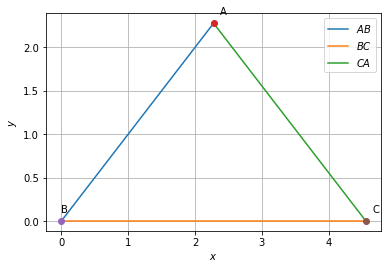
\includegraphics[width=\columnwidth]{solutions/triangle/3/Figure1(2).png}
\caption{$\triangle ABC$}
\label{tri/3/fig:triangle ABC}
\end{figure}


